% Created 2019-11-30 Sat 23:23
% Intended LaTeX compiler: pdflatex
\documentclass[11pt]{article}
\usepackage[utf8]{inputenc}
\usepackage[T1]{fontenc}
\usepackage{graphicx}
\usepackage{grffile}
\usepackage{longtable}
\usepackage{wrapfig}
\usepackage{rotating}
\usepackage[normalem]{ulem}
\usepackage{amsmath}
\usepackage{textcomp}
\usepackage{amssymb}
\usepackage{capt-of}
\usepackage{hyperref}
\author{Heitor Lourenço Werneck \\{\href{mailto:heitorwerneck@hotmail.com}{heitorwerneck@hotmail.com}}}
\usepackage[portuguese]{babel}
\usepackage{mathtools}
\usepackage[binary-units=true]{siunitx}
\usepackage[top=0.5cm,bottom=1.5cm,left=2cm,right=2cm]{geometry}
\usepackage{mdframed}
\usepackage{listings}
\usepackage[noend]{algpseudocode}
\usepackage{algorithm}
\usepackage{tikz}
\usepackage{xcolor}
\usepackage{colortbl}
\usepackage{graphicx,wrapfig,lipsum}
\RequirePackage{fancyvrb}
\DefineVerbatimEnvironment{verbatim}{Verbatim}{fontsize=\small}
\usepackage[font=small,labelfont=bf]{caption} % Required for specifying captions to tables and figures
\usepackage[subrefformat=parens]{subcaption}
\date{\today}
\title{Grafos\\\medskip
\large Trabalho Prático 2}
\hypersetup{
 pdfauthor={Heitor Lourenço Werneck},
 pdftitle={Grafos},
 pdfkeywords={},
 pdfsubject={},
 pdfcreator={Emacs 26.3 (Org mode 9.1.9)}, 
 pdflang={Portuguese}}
\begin{document}

\maketitle
\tableofcontents

\usetikzlibrary{arrows, fit, matrix, positioning, shapes, backgrounds,intersections}
\usetikzlibrary{decorations.pathreplacing}
\usetikzlibrary{automata, positioning, arrows}
\usetikzlibrary{calc}

\definecolor{bg}{rgb}{0.95,0.95,0.95}
\BeforeBeginEnvironment{minted}{\begin{mdframed}[backgroundcolor=bg]}
\AfterEndEnvironment{minted}{\end{mdframed}}
\numberwithin{equation}{section}
\algnewcommand{\IfThenElse}[3]{% \IfThenElse{<if>}{<then>}{<else>}
  \State \algorithmicif\ #1\ \algorithmicthen\ #2\ \algorithmicelse\ #3}

% Define block styles
\tikzstyle{decision} = [diamond, draw, fill=blue!20, 
    text width=4.5em, text badly centered, node distance=3cm, inner sep=0pt]
\tikzstyle{block} = [rectangle, draw, fill=blue!20, 
    text width=5em, text centered, rounded corners, minimum height=4em]
\tikzstyle{line} = [draw, -latex']
\tikzstyle{cloud} = [ellipse, draw, fill=red!20, 
    text width=5em, text centered, rounded corners, minimum height=2em]
%\tikzstyle{cloud} = [draw, ellipse,fill=red!20, node distance=3.5cm,
%    minimum height=2em]


\lstset{
  basicstyle=\ttfamily,
  columns=fullflexible,
  frame=single,
  breaklines=true,
  postbreak=\mbox{\textcolor{red}{$\hookrightarrow$}\space},
}
\DeclarePairedDelimiter\ceil{\lceil}{\rceil}
\DeclarePairedDelimiter\floor{\lfloor}{\rfloor}

\section{Introdução}
\label{sec:org6fbe5d5}
O problema das oito rainhas é um problema comumente usado em ciência da computação para demonstrar o conceito de \emph{backtracking}, o problema consiste em colocar \(n\) rainhas em um tabuleiro de xadrez \(n\times n\) tal que as rainhas não ataquem umas as outras.

Este problema é um caso clássico de um problema de satisfação de condição do campo de inteligência artificial e pesquisa operacional.

Esse problema tem algumas aplicações como por exemplo: controle de tráfego aéreo, teste de VLSI \cite{sosic90_polyn_time_algor_n_queen_probl}, balanceamento de carga \cite{Panwar2013LoadBU} e prevenção de \emph{deadlock} \cite{tanik1978graph}.

Este trabalho visa solucionar esse problema usando uma modelagem em grafos. Também será explorado o problema de n-rainhas.

O problema foi solucionado usando um algoritmo backtracking para busca de soluções e o algoritmo de Bron-Kerbosch para validação de um estado do tabuleiro.

\section{Modelagem e Solução}
\label{sec:org0780497}

Seja N o tamanho do tabuleiro (\(N^2\) é o número de quadrados no mesmo).

O grafo \(G\) que será utilizado para solucionar o problema das rainhas será não direcionado e não ponderado.

Cada posição do tabuleiro \((i,j) \in \{(a,b) : a \in [0,N-1] \land b \in [0,N-1] \}\), que é um quadrado, será mapeado (\(TransformaParaVertice: (i,j) \rightarrow \mathbb{N}\)) para \(i*N+j\), que será um vertice com esse mesmo rótulo.

Logo o grafo \(G(V,E)\) tal que V são os vértices do grafo e E as arestas entre os vértices terá a seguinte propriedade: v \(\in\) V, sendo \(V = \{x \in \mathbb{N} : 0 \leq x \leq N^2-1 \}\)

O mapeamento pode ser visto pelo seguinte tabuleiro \(2\times 2\) (tabela \ref{tab:tabuleiro}) modelado como matriz e a figura \ref{fig:tabgrafos}.

\begin{table}[htbp]
\centering
\begin{tabular}{ll}
\(Quadrado_{00}\) & \(Quadrado_{01}\)\\
\(Quadrado_{10}\) & \(Quadrado_{11}\)\\
\end{tabular}
\caption{\label{tab:tabuleiro}
Tabuleiro modelado na maneira convencional.}

\end{table}


\begin{figure}
\begin{center}
\begin{tikzpicture}[auto,node distance=1.8cm,thick]
\node[state] (0) {0};
\node[state,right of=0] (1) {1};
\node[state,below of=0] (2) {2};
\node[state,below of=1] (3) {3};
\end{tikzpicture}
\end{center}
\caption{Tabuleiro modelado em grafos.}\label{fig:tabgrafos}
\end{figure}

É necessário definir quando existirá uma aresta entre dois vértices. Como o problema em grafos que será utilizado para solucionar o problema das rainhas será o clique, logo o modo que as arestas são dispostas é dependente disso. (Um subconjunto de V(\(V'\subset V\)) será um clique se todos os vértices em \(V'\) estão ligados por uma aresta em \(E\))

Então existirá aresta entre dois vértices se não estiverem na mesma linha, coluna ou diagonal.

Essa solução faz sentido pois o clique terá tamanho \(N\) em uma solução válida pois todas rainhas irão se conectar ja que não estão na mesma linha, coluna ou diagonal. Logo qualquer clique com tamanho \(N\) será uma solução para o problema.

Logo para definir uma regra de criação de arestas será utilizado aritmética modular nos rótulos de cada vértice.

Então dois vértices \(u'\) e \(v'\) terão seus rótulos dados por \(u\) e \(v\) respectivamente e assim a equação \ref{eq:constraints} mostra a condição definida matemáticamente para que seja criado uma aresta.

\begin{equation}
\begin{aligned}
\omega(u,v) = (u\bmod N) \neq (v\bmod N) \land \text{ Não estão na mesma coluna}\\
\floor*{u\div N} \neq \floor*{v\div N} \land \text{ Não estão na mesma linha}\\
(\floor*{u\div N} + u\bmod N) \neq (\floor*{v\div N} + v\bmod N) \land \text{ Não estão na mesma diagonal}\\
(\floor*{u\div N} - u\bmod N) \neq (\floor*{v\div N} - v\bmod N) \text{ Não estão na mesma diagonal}\\
\end{aligned}
\end{equation}\label{eq:constraints}

Logo a criação das arestas será dada pelo algoritmo \ref{alg:insertedge}.

\begin{algorithm}
\textbf{Input:} $G$
\caption{Inserção de arestas.}\label{alg:insertedge}
\begin{algorithmic}[1]
\Procedure{EdgePopulator}{}
\For{$u=0$ to $G.|V|-1$}
\For{$v=0$ to $G.|V|-1$}
\If{$\omega(u,v)$}
\State $G.E \gets G.E \cup \{\{u,v\}\}$ \Comment{Como o grafo é não direcionado então uma aresta será representada por um conjunto ao invés de uma tupla}
\EndIf
\EndFor
\EndFor
\EndProcedure
\end{algorithmic}
\end{algorithm}

Com isso a modelagem do grafo está completa e ele pode ser utilizado para solucionar o problema através do clique.



\subsection{Algoritmo de clique}
\label{sec:org92b554c}

O algoritmo de clique utilizado é o Bron-Kerbosch, esse algoritmo acha todos os cliques maximais de um grafo não direcionado. \cite{bron73_algor}

O algoritmo \ref{alg:bron-kerbosch} descreve o comportamento detalhado. A escolha do pivo foi feita pelo vértice com maior grau. A complexidade de tempo do algoritmo tradicional de acordo com a literatura é \(O(3^{\frac{n}{3}})\).

\begin{algorithm}
\textbf{Input:} $G$
\caption{Algoritmo de busca de cliques maximais.}\label{alg:bron-kerbosch}
\begin{algorithmic}[1]
\Procedure{Bron-Kerbosch}{$R,P,X,degrees,N,maximal\_cliques$}
\If{$P = \emptyset \land X = \emptyset $}
\State $maximal\_cliques \gets maximal\_cliques \cup \{R\}$
\State \textbf{return}
\EndIf
\State $u \gets argmax_{v\in P \cup X} degrees[v]$
\For{$v$ in $P\setminus N[u]$}
\State Bron-Kerbosch($R \cup \{v\}$,$P \cap N[v]$,$X \cap N[v],degrees,N,maximal\_cliques$)
\State $P \gets P \setminus \{v\}$
\State $X \gets X \cup \{v\}$
\EndFor
\EndProcedure
\Procedure{MaximumClique}{$G$}
\State $maximal\_cliques \gets \emptyset$
\State Bron-Kerbosch($\emptyset,G.V,\emptyset,G.degrees,G.neighbors,maximal\_cliques$)
\State \textbf{return} $max_{c \in maximal\_cliques} |c|$
\EndProcedure
\end{algorithmic}
\end{algorithm}


Então com o algoritmo de clique definido é possivel verificar a validade de uma combinação de rainhas.

\subsection{Backtracking}
\label{sec:org6779e96}

Com a base feita pode-se solucionar o problema, basta fazer uma busca pelas soluções. A escolha foi fazer um algoritmo de backtracking tal que tenta colocar rainhas em diversas disposições e se uma disposição não for válida ela não será explorada mais profundamente. O algoritmo \ref{alg:solvenqueens} descreve detalhadamente o comportamento da solução.

\begin{algorithm}
\textbf{Input:} $G$
\caption{Algoritmo de busca das soluções do problema de N rainhas.}\label{alg:solvenqueens}
\begin{algorithmic}[1]
\State $solutions \gets \emptyset$
\Procedure{SolveNQueens}{$column,G,queens$}
\If{$column = N$}
\State $solutions\gets solutions \cup \{queens\}$
\State \textbf{return}
\EndIf
\For{$current\_row=0$ \textbf{to} $N-1$}
\State $vertex \gets column+current\_row\cdot N$
\State $new\_queens\_set \gets queens \cup \{vertex\}$
\State $sub\_graph \gets G.subgraph(new\_queens\_set)$\Comment{Grafo induzido com os vértices do conjunto}
\If{$MaximumClique(sub\_graph) = column+1$}\Comment{Checa validade do conjunto de rainhas}
\State SolveNQueens($column+1,G,new\_queens\_set)$
\EndIf
\EndFor
\EndProcedure
SolveNQueens($0,G,\emptyset$)
\end{algorithmic}
\end{algorithm}


\section{Análise de resultados}
\label{sec:orgfa1feab}

Os parâmetros que fazem sentido serem variados são o tamanho do tabuleiro juntamente com a quantidade de rainhas.

Primeiro a tabela \ref{tab:data} mostra as soluções obtidas para diversas quantidades de rainhas.

\begin{table}[htbp]
\centering
\begin{tabular}{rrr}
Rainhas & \#Soluções & Tempo(s)\\
\hline
1 & 1 & 0.0001\\
2 & 0 & 0.00035\\
3 & 0 & 0.0011\\
4 & 2 & 0.00475\\
5 & 10 & 0.0254\\
6 & 4 & 0.1456\\
7 & 40 & 0.8206\\
8 & 92 & 5.0287500000000005\\
9 & 352 & 32.9279\\
10 & 724 & 208.9649\\
11 & 2680 & 1473.8914\\
\hline
\end{tabular}
\caption{Resultados.\label{tab:data}}

\end{table}

Primeiramente é possivel notar que as soluções são compativeis com a literatura. \cite{erbas92_differ_n_queen}

Uma parte importante sobre o número de soluções é que algumas são rotações de outras soluções, no caso do problema das 8 rainhas existem 12 soluções únicas. \cite{erbas92_differ_n_queen}

Outro ponto a se notar é que o problema das rainhas está sendo resolvido com dois algoritmos de complexidade exponencial, o \emph{backtracking} e o algoritmo de clique que faz parte do \emph{backtracking}, isso torna o algoritmo pouco eficiente tanto que não foi possível executar para 12 rainhas.

Na figura \ref{fig:time} é possivel ver que o crescimento do tempo em função do tamanho do número de rainhas é exponencial, comprovando assim a hipótese anterior de que sua complexidade é exponencial.

Pela figura \ref{fig:solution} é possível ver o crescimento da quantidade de soluções, entre o problema de 1 e 6 rainhas o crescimento é instável pela própria estrutura do problema, poŕem após isso o crescimento é de pelo menos o dobro de soluções.

\begin{figure}[htbp]
\centering
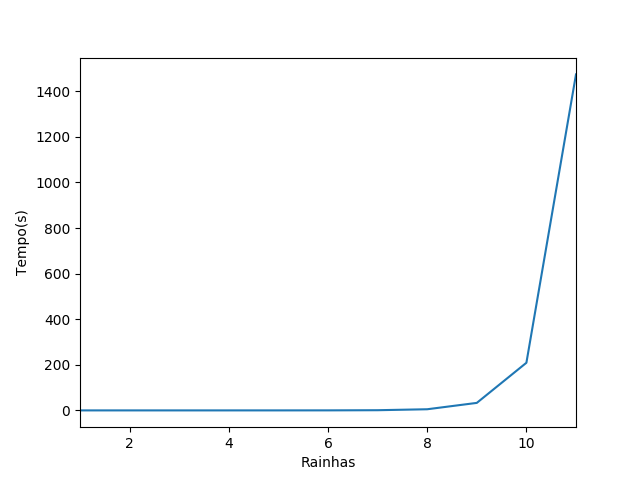
\includegraphics[width=.9\linewidth]{time.png}
\caption{\label{fig:time}
Tempo de execução por número de rainhas.}
\end{figure}



\begin{figure}[htbp]
\centering
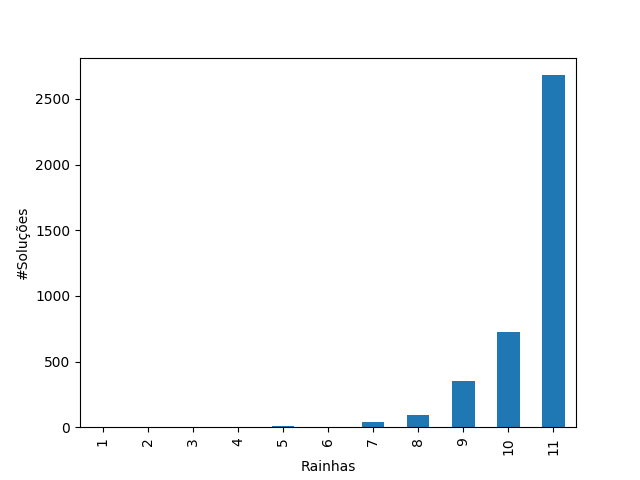
\includegraphics[width=.9\linewidth]{num_solutions.png}
\caption{\label{fig:solution}
Soluções por número de rainhas.}
\end{figure}



\section{Conclusão}
\label{sec:orgeae9eef}

Com esse trabalho foi possível entender que modelando o problema com grafos e resolvendo o mesmo com um algoritmo de um problema NP-Difícil torna o algoritmo muito ineficiente, fora o \emph{overhead} da manipulação das estruturas que representam um grafo.

Porém também foi possível pensar em novas abordagens para se solucionar o problema das 8 rainhas, em trabalhos futuros seria interessante solucionar o mesmo com outros algoritmos de grafos, buscando o mais eficiente em termos de compĺexidade assintótica de tempo.

Os resultados obtidos do número de soluções foram iguais a literatura o que checa a validade da solução em partes.


\bibliographystyle{plain}
\bibliography{doc}
\end{document}
